\documentclass[11pt]{beamer}

\usetheme{Darmstadt}
\usepackage{tikz}
\usepackage{amsmath,amssymb}

% Define colors
\definecolor{lightblue}{RGB}{120, 200, 230}
\definecolor{darkblue}{RGB}{30, 100, 130}
\definecolor{lightgray}{RGB}{150, 150, 150}
\definecolor{darkgray}{RGB}{70, 70, 70}

\begin{document}

\begin{frame}
\frametitle{Probabilidade Condicional}

$p(B|A)$ denota a probabilidade de ocorrência de $B$ dado que $A$ ocorreu.

Esta probabilidade pode ser calculada usando o teorema de Bayes:

$$p(A\cap B)=p(B|A)p(A)=p(A|B)p(B)$$

\begin{center}
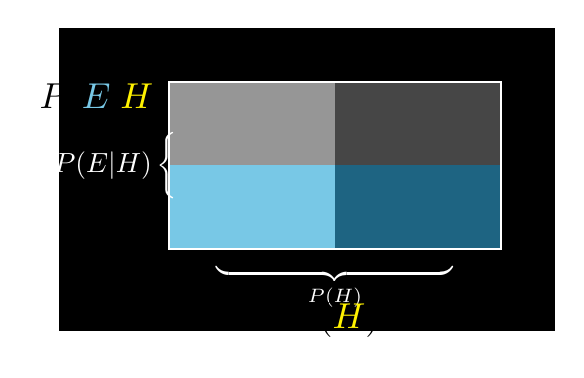
\begin{tikzpicture}[scale=.7]
    % Fundo preto
    \fill[black] (-2,-1.5) rectangle (7,4);
    
    % Retângulo principal (espaço amostral)
    \draw[white, very thick] (0,0) rectangle (6,3);
    
    % Divisão interna do retângulo
    \draw[white, very thick] (3,0) -- (3,3);
    \draw[white, very thick] (0,1.5) -- (6,1.5);
    
    % Preenchimento das áreas
    \fill[lightgray] (0,1.5) rectangle (3,3);
    \fill[lightblue] (0,0) rectangle (3,1.5);
    \fill[darkgray] (3,1.5) rectangle (6,3);
    \fill[darkblue] (3,0) rectangle (6,1.5);
    
    % Rótulos P(E|H)
    \node[white] at (-0.7,1.5) {$P(E|H) \left\{\begin{array}{c} \\ \\ \end{array}\right.$};
    
    % Rótulos P(H)
    \node[white] at (3,-0.7) {$\underbrace{\hspace{3cm}}_{P(H)}$};
    
    % Texto E e H em cores diferentes
    \node[scale=1.3] at (-1.2,2.7) {$P($\textcolor{lightblue}{$E$}$|$\textcolor{yellow}{$H$}$)$};
    
    % Texto H em cor diferente no termo P(H)
    \node[scale=1.3] at (3,-1.3) {$P($\textcolor{yellow}{$H$}$)$};
\end{tikzpicture}
\end{center}

\vspace{0.5cm}
\begin{alertblock}{Teorema de Bayes}
\begin{align}
P(A|B) = \frac{P(B|A) \cdot P(A)}{P(B)}
\end{align}

\begin{align}
P(\textcolor{lightblue}{E}|\textcolor{yellow}{H}) = \frac{P(\textcolor{yellow}{H}|\textcolor{lightblue}{E}) \cdot P(\textcolor{lightblue}{E})}{P(\textcolor{yellow}{H})}
\end{align}
\end{alertblock}
\end{frame}

\end{document}
